%%%% Paramétrage du TD %%%%
\def\xxactivite{TD 01 \ifprof -- Corrigé \else \fi }
\def\xxauteur{\textsl{Xavier Pessoles}}


\def\xxnumchapitre{Chapitre 1 \vspace{.2cm}}
\def\xxchapitre{\hspace{.12cm} Stabilité des systèmes}

\def\xxcompetences{%
\textsl{%
\textbf{Savoirs et compétences :}\\
\vspace{-.4cm}
\begin{itemize}[label=\ding{112},font=\color{bleuxp}] 
%\item \textit{Mod3.C2 : } pôles dominants et réduction de l’ordre du modèle : principe, justification
%\item \textit{Res2.C4 : } stabilité des SLCI : définition entrée bornée -- sortie bornée (EB -- SB)	
%\item \textit{Res2.C5 : } stabilité des SLCI : équation caractéristique	
\item \textit{Res2.C6 : } stabilité des SLCI : position des pôles dans le plan complexe
\item \textit{Res2.C7 : } stabilité des SLCI : marges de stabilité (de gain et de phase)
\end{itemize}
}}


\def\xxfigures{
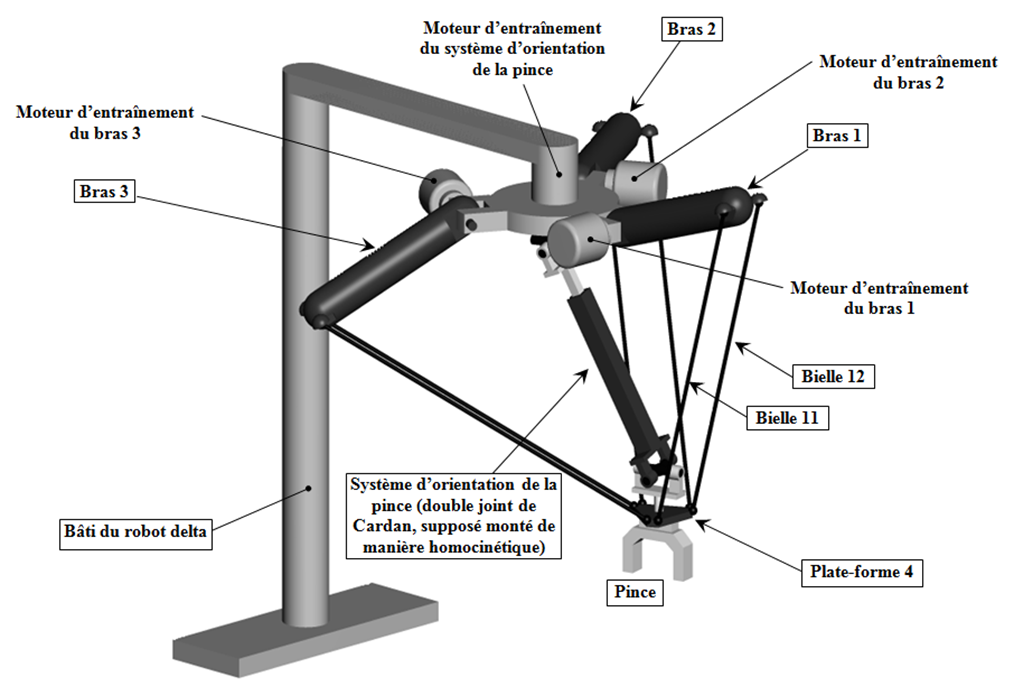
\includegraphics[width=.9\linewidth]{fig_01}
}%figues de la page de garde

\def\xxtitreexo{Drone quadri-rotor}
\def\xxsourceexo{\hspace{.2cm} \footnotesize{\textsl{Pole SII Chateaubriand -- Joliot Curie}}}


\iflivret
\input{\repRel/Style/pagegarde_TD}
\else
\input{\repRel/Style/pagegarde_TD}
\fi
\setlength{\columnseprule}{.1pt}

\pagestyle{fancy}
\thispagestyle{plain}


\vspace{4.5cm}

\def\columnseprulecolor{\color{bleuxp}}

%%%%%%%%%%%%%%%%%%%%%%%


\ifprof
\else
\begin{multicols}{2}
\fi
\setcounter{numques}{0}
\section*{Présentation}
\ifprof
\else
Cet hélicoptère quadri-rotor à pas fixe est une configuration très répandue dans le monde des microdrones.
Alors que les hélicoptères classiques utilisent un système mécanique complexe de pas cyclique et
collectif, le quadri-rotor ne dispose d'aucun organe mécanique spécifique et assure son contrôle en agissant
uniquement sur la vitesse de rotation de ses rotors. Cette simplicité permet de disposer d'un engin de faible
coût, robuste et facile à miniaturiser.
Le contrôle vertical de l'appareil (translation suivant la direction $\vect{z}$) est obtenu en faisant varier
simultanément la vitesse de rotation des quatre moteurs. Le contrôle en roulis (rotation autour de l’axe $(O,\vect{x})$ ) et en tangage (rotation autour de l’axe $(O,\vect{y})$ ) est obtenu en faisant varier de manière différentielle
les vitesses de rotation des moteurs d'un même axe ($\dfrac{\omega_2}{\omega_4}$  pour le roulis et $\dfrac{\omega_1}{\omega_3}$ pour le tangage).
Un extrait du cahier des charges en phase de décollage est donné ci-dessous.


\begin{center}
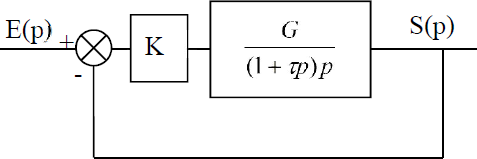
\includegraphics[width=\linewidth]{fig_02}
\end{center}
\fi
\begin{obj}
\begin{itemize}
\item Étudier le comportement du quadri-rotor lors du décollage.
\item Vérifier les performances imposées par le cahier des charges.
\end{itemize}
\end{obj}

\section*{Linéarisation du modèle de moteur}
\ifprof
\else

Les moteurs choisis sont des moteurs synchrones sans balais à 14 pôles de type Hacker A20-54 entraînant
directement l'hélice, sans réduction.

\begin{center}
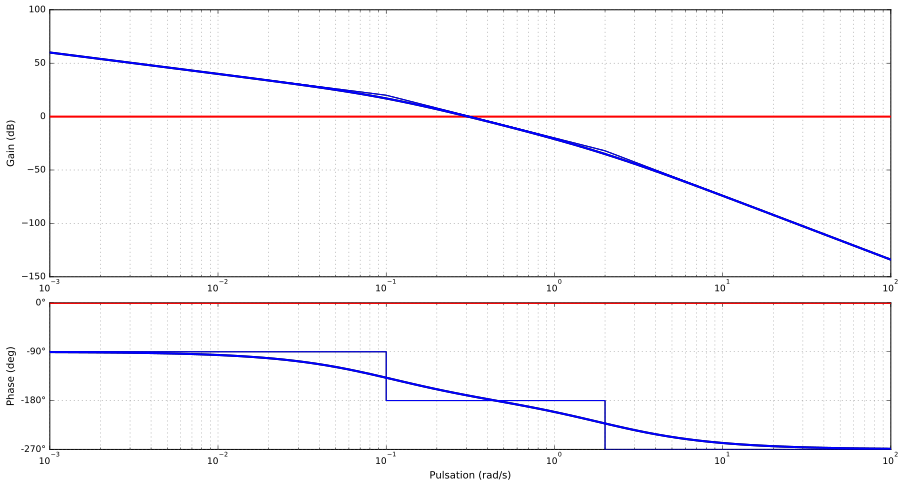
\includegraphics[width=.4\linewidth]{fig_03}
\end{center}

Sous certaines hypothèses simplificatrices, l'équation globale modélisant le moteur et sa commande peut se
mettre sous la forme suivante :
$$
\dfrac{\text{d}\omega(t)}{\text{d}t}=-\dfrac{1}{\tau}\omega(t) -k_q\omega(t)^2 + \dfrac{k_v}{\tau}u.
$$

$u$ représente la tension de commande du moteur, $\omega(t)$ son taux de rotation, $\tau$ et $k_v$ des constantes caractéristiques de l'ensemble moteur-hélice. Le terme $k_q\omega^2$ provient du couple de frottement aérodynamique de l'air sur l'hélice tournant à grande vitesse.

L'équation du modèle du moteur fait apparaître un terme non linéaire en $\omega^2$, qui nécessite de linéariser
donc l'équation autour du point de fonctionnement $\omega_0$, fréquence de rotation du moteur qui permet de
maintenir le mini-drone en équilibre en vol stationnaire.

On pose $\omega=\omega_0+\delta \omega$ et $u=u_0+\delta u$ où $\delta\omega$ et $\delta u$ représentent des petites variations de $\omega$ et $u$ autour du point de fonctionnement.
\fi

\question{Déterminer l’équation stationnaire liant $\omega_0$ et $u_0$.}
\ifprof
\begin{corrige}
En vol stationnaire, dans les conditions idéales, la vitesse de rotation des hélices est constante; donc $\dfrac{\dd \omega(t)}{\dd t} = 0$. De plus, il n'y a pas de variation de la vitesse de rotation des hélices et donc pas de variation de la tension d'alimentation. En conséquence, $\delta u =0$ et $\delta \omega = 0$.

On a donc 
$
\dfrac{\text{d}\omega(t)}{\text{d}t}=-\dfrac{1}{\tau}\omega(t) -k_q\omega(t)^2 + \dfrac{k_v}{\tau}u $ 
En notant $\omega_0$ et $u_0$ les vitesses en tensions à l'état stationnaire, on a 
$\dfrac{1}{\tau}\omega_0 +k_q\omega_0^2 = \dfrac{k_v}{\tau}u_0$.

\end{corrige}
\else
\fi

\question{Montrer que l'équation différentielle liant $\delta \omega$ et $\delta u$ est de la forme $\dfrac{\text{d}\delta \omega(t) }{\text{d}t}=-A\delta \omega(t) + B \delta u$. Exprimer $A$ et $B$ en fonction des paramètres $\tau$, $k_v$, $k_q$ et $\omega_0$.}
\ifprof
\begin{corrige}
On utilise le changement de variable proposé autour d'un point de fonctionnement et on a : 
$
\dfrac{\text{d}\omega(t)}{\text{d}t}=-\dfrac{1}{\tau}\omega(t) -k_q\omega(t)^2 + \dfrac{k_v}{\tau}u
$

$
\Rightarrow 
\dfrac{\text{d}\left( \omega_0+\delta \omega \right)}{\text{d}t}=-\dfrac{1}{\tau}\left( \omega_0+\delta \omega\right) -k_q\left( \omega_0+\delta\omega \right)^2 + \dfrac{k_v}{\tau}\left( u_0+\delta u\right)
$

$
\Rightarrow 
\dfrac{\text{d}\left(\delta \omega \right)}{\text{d}t}=-\dfrac{1}{\tau} \omega_0-\dfrac{1}{\tau}\delta \omega -k_q \omega_0^2-k_q\left(\delta\omega\right)^2 -k_q2 \omega_0 \delta\omega + \dfrac{k_v}{\tau} u_0+\dfrac{k_v}{\tau} \delta u
$

Or $\dfrac{1}{\tau}\omega_0 +k_q\omega_0^2 = \dfrac{k_v}{\tau}u_0$ (question précédente); donc :
$
\dfrac{\text{d}\left(\delta \omega \right)}{\text{d}t}= -\dfrac{1}{\tau}\delta \omega-k_q\left(\delta\omega\right)^2 -k_q2 \omega_0 \delta\omega + \dfrac{k_v}{\tau} \delta u
$

En négligeant les termes d'ordre 2, on a donc : 
$
\dfrac{\text{d}\left(\delta \omega \right)}{\text{d}t}= -\dfrac{1}{\tau}\delta \omega -k_q2 \omega_0 \delta\omega + \dfrac{k_v}{\tau} \delta u
$

Au final, $A=\dfrac{1}{\tau}+k_q2 \omega_0$ et $B=\dfrac{k_v}{\tau}$.
\end{corrige}
\else
\fi
On note $\Delta \Omega (p)$ la transformée de Laplace de $\delta \omega$ et $\Delta U(p)$ celle de $\delta u$.


\question{Calculer la fonction de transfert $\dfrac{\Delta{\Omega(s)}}{\Delta U(s)}$ du moteur. Donner l'expression de ses paramètres caractéristiques $K_m$ et $T_m$ en fonction des paramètres $\tau$, $k_v$, $k_q$ et $\omega_0$.}
\ifprof
\begin{corrige}
En utilisant la transformée de Laplace, on obtient $p\Delta\Omega(s) = -A\Delta\Omega(s) + B \Delta U(s)$ et donc 
 $\dfrac{\Delta{\Omega(s)}}{\Delta U(s)}= \dfrac{B}{p+A} = \dfrac{B/A}{p/A+1}  $. 
 En conséquence, $K_m = \dfrac{B}{A} = \dfrac{\dfrac{k_v}{\tau}}{\dfrac{1}{\tau}+k_q2 \omega_0}= \dfrac{k_v}{1+\tau k_q2 \omega_0}$. 
 $\tau_m = \dfrac{\tau}{1+\tau k_q2 \omega_0} $ 
\end{corrige}
\else
\fi
\section*{Recherche du point de fonctionnement $\omega_0$}
\ifprof
\else
Dans le mouvement de déplacement vertical de direction $\vect{z}$ , les quatre moteurs tournent à la même vitesse et fournissent la même poussée $F=F_1=F_2=F_3=F_4$.
La masse totale du drone est $m=\SI{240}{g}$. On prendra $g=\SI{9,81}{m.s^{-2}}$.
\fi


\question{Calculer numériquement la poussée $F_0$ que doit exercer chacun des quatre moteurs pour maintenir l’appareil en vol stationnaire à l’altitude $z_0$ .}
\ifprof
\begin{corrige}
On a  $4 F_0 = mg$. 
Le poids du drone est de $0,240\times 9,81 = \SI{2,3544}{N}$. Chaque moteur doit donc exercer $\dfrac{2,3544}{4}=\SI{0,59}{N}$.
\end{corrige}
\else
\fi
\ifprof
\else
La poussée $F$ varie avec $\omega^2$ . Des mesures réalisées sur un seul groupe moteur-hélice ont permis de tracer la courbe liant $F$ à la fréquence de rotation $\omega$ en rad/s.

\begin{center}
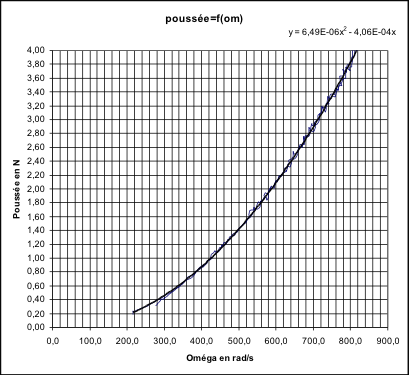
\includegraphics[width=\linewidth]{fig_04}
\end{center}

\fi

\question{Déterminer la fréquence de rotation $\omega_0$ des
moteurs en vol stationnaire.}
\ifprof
\begin{corrige}
En lisant le graphe, on obtient $\omega_0=\SI{340}{rad.s^{-1}}$.
\end{corrige}
\else
\fi

\ifprof
\else

Des essais ont également permis de tracer la
courbe liant la tension de commande $u$ et la
fréquence de rotation $\omega$ en rad/s en régime
permanent lorsque $\dfrac{\text{d}\omega(t)}{\text{d}(t)}=0$. La courbe de tendance associée aux résultats de
ces essais est de la forme $y=ax^2+bx$. On donne la constante de temps du moteur :
$\tau=\SI{125}{ms}$.

\begin{center}
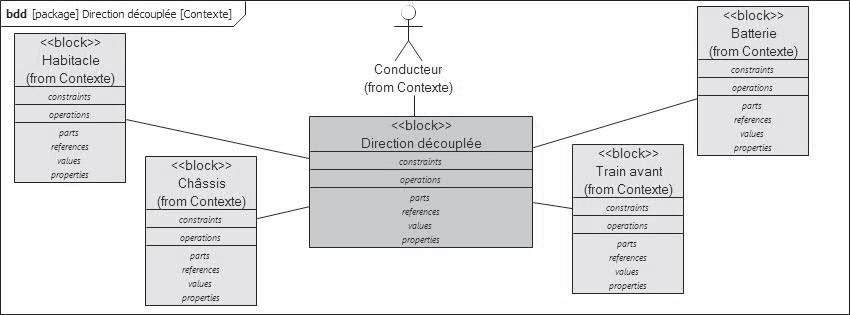
\includegraphics[width=\linewidth]{fig_05}
\end{center}
\fi

\question{Déterminer l'expression des coefficients $k_v$ et $k_q$ en fonction de $a$, $b$ et $\tau$. Préciser leur unité.}
\ifprof
\begin{corrige}
Lorsque $\dfrac{\text{d}\omega(t)}{\text{d}(t)}=0$, on a  $u=a\omega0^2+b\omega_0$. Par ailleurs en régime stationnaire, on a $\dfrac{1}{\tau}\omega_0 +k_q\omega_0^2 = \dfrac{k_v}{\tau}u_0$. Il en résulte que 
$u_0 = \dfrac{1}{k_v}\omega_0 +\dfrac{k_q\tau}{k_v} \omega_0^2$.

On a donc $a=\dfrac{k_q\tau}{k_v}$ et  $b=\dfrac{1}{k_v}$. On a donc $b$ tel que $[\text{V}]=[\text{B}][\text{s}^{-1}]$ et $[\text{B}]=[\text{V}][\text{s}]$. On a donc $k_v$ en $[\text{V}^{-1}\text{s}^{-1}]$.

Par ailleurs, $[\text{V}]=[\text{k}_{\text{q}}][\text{s}][\text{Vs}][\text{s}^{-2}]$  et $k_q$ n'a pas d'unité. 

\end{corrige}
\else
\fi

On peut ainsi déduire le modèle $\dfrac{\Delta \Omega(p)}{\Delta U(p)}$ du moteur linéarisé autour de son point de fonctionnement. Pour la suite, on retiendra le modèle suivant : $\dfrac{\Delta \Omega(p)}{\Delta U(p)}=\dfrac{37,5}{1+\dfrac{p}{77}}$.

\section*{Vérification des performances}

\ifprof
\else
L'asservissement vertical du drone peut être représente après linéarisation des différentes fonctions de
transfert autour du point de fonctionnement $\omega_0$, par le schéma-bloc suivant :

\begin{center}
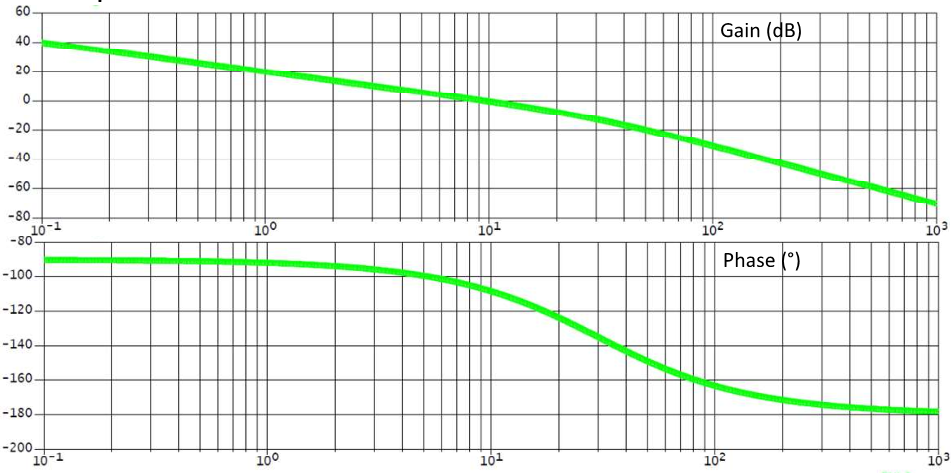
\includegraphics[width=\linewidth]{fig_06}
\end{center}



Le gain du capteur barométrique est de $\SI{0,05}{V.m^{-1}}$. On pose $z(t)=z_0+\delta z(t)$, $\Delta Z(p)$ la transformée de Laplace de $\delta z(t)$, $F=F_0 + \delta F$ représente la poussée d'un seul moteur et on utilise l'équation linéarisée avec conditions initiales nulles.

Le théorème de la résultante dynamique, en projection sur l’axe vertical, permet d’écrire :
$$ m\ddot{z} =4F-mg. $$
\fi


\question{Déterminer la fonction de transfert $\dfrac{\Delta Z(p)}{\Delta F(p)}$ à partir de l'équation du principe fondamental de la dynamique. En déduire l'expression de la fonction de transfert en boucle ouverte. }

\ifprof
\begin{corrige}
On a vu que  $4 _0F = mg$. 

Par ailleurs, $ m\ddot{z} =4F-mg $ et donc, $ m\dfrac{ \dd\left( z_0+\delta z(t) \right)}{\dd t} = 4\left( F_0 + \delta F(t) \right)-mg$ et
 $ m\dfrac{ \dd\left( \delta z(t) \right)}{\dd t} = 4 \delta F(t) $. Dans le domaine de Laplace, on a 
  $ m p^2  \Delta Z(p) = 4 \Delta F(p) $. En conséquences,  
   $\dfrac{\Delta Z(p)}{\Delta F(p)} = \dfrac{4}{mp^2}$.
   
La FTBO s'exprime alors par $H_{\text{BO}}(p)=\dfrac{2,5 K}{p^2}\dfrac{1+Tp}{\left( 1+\dfrac{p}{77}\right)\left(1+\dfrac{p}{30} \right)}$.
\end{corrige}
\else
\fi

\ifprof
\else
Dans la suite, le gain de la fonction de transfert en boucle ouverte sera noté $K_{BO}=2,5 K$.
La courbe de phase du diagramme de Bode de la fonction de transfert en boucle ouverte est représentée ci-dessous, en gras avec un correcteur proportionnel ($T=0$) et en trait fin avec le correcteur retenu ($K=1$ et $T=0,2s$).


\begin{center}
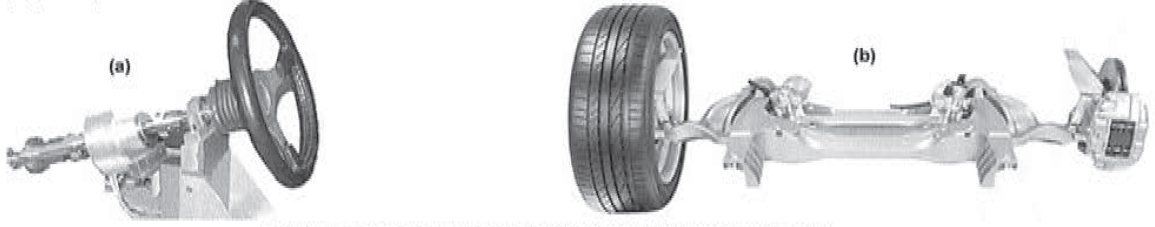
\includegraphics[width=\linewidth]{fig_07}
\end{center}
\fi


\question{Tracer le diagramme asymptotique de la courbe de gain avec le correcteur $T=\SI{0,2}{s}$ et $K=1$.
Préciser les pentes et les pulsations de brisure. Le diagramme sera tracé entre 1 et \SI{1000}{rad.s^{-1}}, le gain sera compris entre \SI{-120}{dB} et \SI{+10}{dB}.}

\ifprof
\begin{corrige}
On a  $H_{\text{BO}}(p)=\dfrac{2,5 K}{p^2}\dfrac{1+Tp}{\left( 1+\dfrac{p}{77}\right)\left(1+\dfrac{p}{30} \right)}$. 
Les pulsations de cassure sont alors :  $\SI{5}{rad.s^{-1}}$, $\SI{30}{rad.s^{-1}}$ et $\SI{77}{rad.s^{-1}}$.
Les pentes sont alors : 
\begin{itemize}
\item pour $\omega<\SI{5}{rad.s^{-1}}$ : \SI{-40}{dB}/décade;
\item pour $\SI{5}{rad.s^{-1}}<\omega<\SI{30}{rad.s^{-1}}$ : \SI{-20}{dB}/décade;
\item pour $\SI{30}{rad.s^{-1}}<\omega<\SI{77}{rad.s^{-1}}$ : \SI{-40}{dB}/décade
\item pour $\omega>\SI{77}{rad.s^{-1}}$ : \SI{-60}{dB}/décade.
\end{itemize}
Pour une pulsation de $\SI{10e-2}{rad.s^{-1}}$, on a $\text{FTBO(p)}\simeq \dfrac{2,5}{p^2}$. On a donc un gain $\simeq 20\log\left(\dfrac{2,5}{0,01^2}\right) \simeq \SI{88}{dB} $.
Reste à tracer...
\end{corrige}

\fi

\question{Justifier que pour $K=1$, on a $\omega_{c\SI{0}{dB}}=\SI{1,5}{rad.s^{-1}}$. En déduire graphiquement la marge de phase pour
$K=1$. Commenter.}
\ifprof
\begin{corrige}
Si on considère que pour $\omega<\SI{5}{rad.s^{-1}}$, on a   $H_{\text{BO}}(p)\simeq \dfrac{2,5 K}{p^2}$. Dans ces conditions, pour $K=1$, on a 
$\left|\dfrac{2,5 }{-\omega^2}\right|=1$ 
$\Rightarrow \omega= \sqrt{2,5}\simeq \SI{1,58}{rad.s^{-1}} $.

\end{corrige}
\else
\fi


\question{Procéder au réglage du gain $K$ du correcteur afin d’assurer le respect du critère de stabilité du cahier des charges.}
\ifprof
\begin{corrige}
En raisonnant analytiquement, on cherche la pulsation $\omega_{-145}$ pour laquelle la phase est de $-180\degres+35\degres = -145\degres$, soit $\arg{\text{FTBO}(j\omega)}=-145\degres$. (Résolution à faire à la calculatrice, sur Python ou autre. Il y asurement 2 solutions vu le profil de courbe de phase). 
On cherche ensuite $K$ tel que $\left| \text{FTBO}(j\omega_{-145}) \right| = 1$. 
(Résolution à faire à la calculatrice, sur Python ou autre.)
\end{corrige}
\else
\fi

\question{Le critère de précision du cahier des charges est-il vérifié ? Justifier.}
\ifprof
\begin{corrige}
La boucle ouverte comporte 2 intégrateurs. L'écart statique est donc nul. Le cahier des charges est vérifié. 

\end{corrige}
\else
\fi

\ifprof
\else

La figure suivante représente la position des pôles de la fonction de transfert en boucle fermée dans le plan
complexe, pour la valeur du gain $K$ précédemment déterminée.


\begin{center}
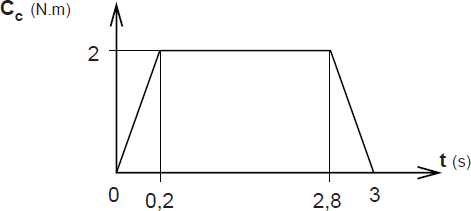
\includegraphics[width=\linewidth]{fig_08}
\end{center}
\fi


\question{Repérer le(s) pôle(s) dominant(s) et donner sa (leur) valeur(s) numérique(s).}
\ifprof
\begin{corrige}
Les pôles dominants sont $P2\simeq -15$, $P3 \simeq -5 +8i$, $P4\simeq -5 -8i$. 
\end{corrige}
\else
\fi

\question{À l’aide des droites d’iso-amortissement, indiquer la valeur du coefficient d’amortissement $\xi$ de la
fonction de transfert du deuxième ordre pouvant modéliser l’asservissement vertical du drone lorsque
l’on néglige les autres pôles par rapport à ces pôles dominants.}
\ifprof
\begin{corrige}
Dans ce cas, on ne prend que $P3$ et $P4$. $\xi=0,6$. 
\end{corrige}
\else
\fi

\question{En déduire la présence ou l’absence d’oscillations verticales du drone lors d’un décollage supposé
modélisé par un échelon d’amplitude 1 mètre. Le critère de stabilité est-il intégralement vérifié ?}
\ifprof
\begin{corrige}
Le coefficient d'amortissement est inférieur à 0,69. Il y aura donc des oscillations verticales lors du drone. Le dépassement sera supérieur à 5\,\% de la valeur finale.  En conséquence, le critère de stabilité n'est pas totalement respecté. 
\end{corrige}
\else
\fi

\question{Donner l’expression littérale des pôles d’un système du deuxième ordre de pulsation propre $\omega_n$ et de coefficient d’amortissement $\xi<1$. En déduire une estimation de la pulsation propre $\omega_n$ de la
fonction de transfert approchée de l’asservissement vertical du drone.}
\ifprof
\begin{corrige}
\end{corrige}
\else
\fi

\question{Vérifier si le critère de rapidité du cahier des charges est vérifié.}
\ifprof
\begin{corrige}
\end{corrige}
\else
\fi

\ifprof
\else
\begin{center}
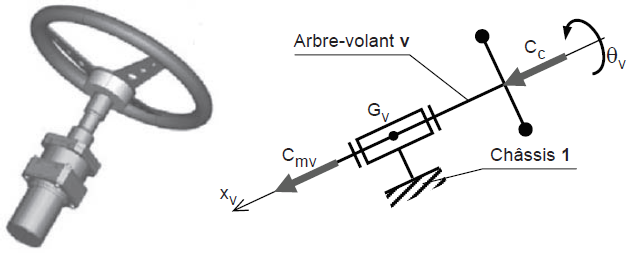
\includegraphics[width=\linewidth]{fig_09}
\end{center}
\fi


%\begin{multicols}
%\newpage

\ifprof
\else
\begin{tabular}{|p{.95\linewidth}|}
\hline
\footnotesize
Pour éventuellement vous aider....
\begin{enumerate}
\item $-\dfrac{1}{\tau}\omega_0 - k_q \omega_0^2 + \dfrac{k_v}{\tau}u_0=0$;
\item $A=\dfrac{1}{\tau}+2k_q\omega_0$ et $B=\dfrac{k_v}{\tau}$.
\item $K_m=\dfrac{k_v}{1+2\tau k_q \omega_0}$ et $T_m=\dfrac{\tau}{1+2\tau k_q \omega_0}$.
\item $F_0=\dfrac{mg}{4}=\SI{0,6}{N}$.
\item $\omega_0=\SI{340}{rad.s^{-1}}$.
\item $k_v=\dfrac{1}{b}$ (rad/s/V) et $k_b=\dfrac{a}{b\tau}$.
\item $\dfrac{\Delta Z(p)}{\Delta F(p)}=\dfrac{4}{mp^2}$. $H_{BO}(p)=\dfrac{2,5 K}{p^2}\dfrac{1+Tp}{\left( 1+\dfrac{p}{77}\right)\left(1+\dfrac{p}{30} \right)}$.
\item  $\quad$
\item $\quad$
\item $K=17,9$.
\item La FTBO est de classe 2, l'erreur de position est donc nulle.
\item $p_2=-15$, $p_3 = -5+8j$, $p_4=-5+8j$.
\item $\xi=0,6$
\item $\quad$
\item $p=-\xi\omega_n \pm j\omega_n \sqrt{1-\xi^2}$. $\omega_n\simeq \SI{8,33}{rad.s^{-1}}$
\item $t_{5\%}\simeq \SI{0,61}{ s}$. 
\end{enumerate} \\ \hline
\end{tabular}
\normalsize
\fi

\ifprof
\else
\end{multicols}

\fi
%\end{document}
%
%\question{}
%
%
%\begin{center}
%\includegraphics[width=\linewidth]{}
%\end{center}
%
%\begin{center}
%\includegraphics[width=\linewidth]{}
%\textit{}
%\end{center}
%
